	\begin{figure}[!bhp]
	\centering
		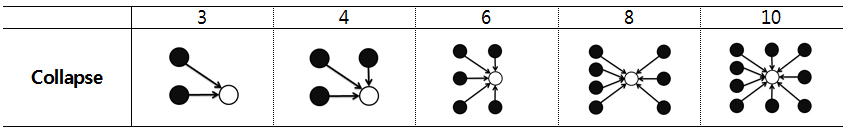
\includegraphics[height=50pt]{Topologies_Collapse}
		\caption{Bayesian Network Topology : Collapse}
	\end{figure}	

	% Collapse는 한 개의 자식 node에 여러 개의 부모 노드가 존재하는 형태이다.
	Collapse is a form in which a plurality of parent nodes are present in one child node.

	\begin{figure}[!bhp]
	\centering
		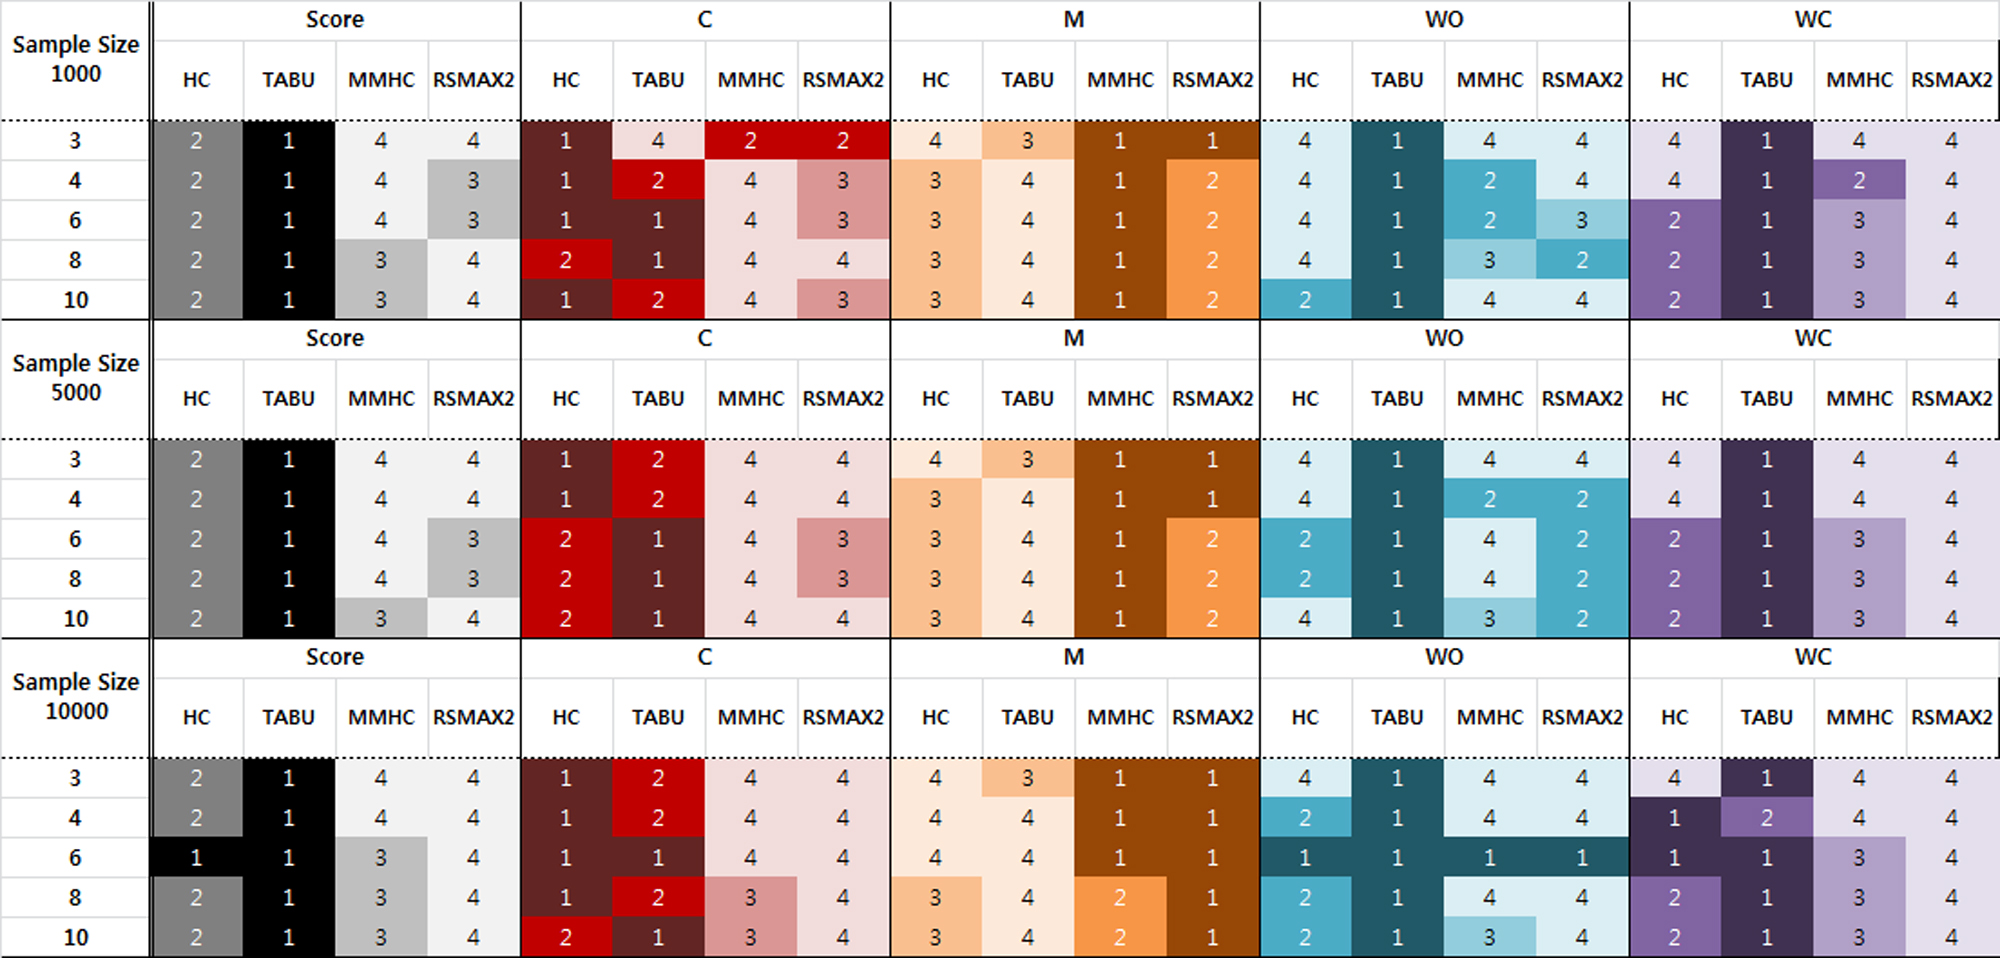
\includegraphics[height=170pt]{Result_Collapse}
		\caption{Summary for Comparison via Collapse}
	\end{figure}	
	
% Real data set을 이용하여 분석할 때와 마찬가지로, score를 기준으로 하였을 때 TABU search 알고리즘, Hill-climbing 알고리즘 순으로 성능이 좋은 것으로 나타났다.
The same way that you were analyzed using the Real data set, TABU search algorithm when it is on the basis of the score, in the order of the Hill-climbing algorithm performance is found to be good.

% 그러나 C의 개수는 TABU search와 Hill-climbing이 서로 경합을 벌였다. 오히려 TABU search의 경우 WO, WC의 개수가 많이 나타났다.
However, the number of C is, TABU search and Hill-climbing has been engaged in a conflict with each other. Rather the case of TABU search WO, became a lot number of WC.

% Hill-climbing의 경우 TABU search만큼은 아니지만, node의 개수가 많아질수록, sample size가 커질수록 WO의 개수가 많아지는 현상이 나타났다.
Not as much as TABU search case of Hill-climbing, The more the number of node, sample size appeared many made phenomenon is the number of larger the WO.

% MMHC는 sample size가 커질수록 missing이 줄어드는 반면, RSMAX2는 오히려 늘어나는 현상이 나타났다.
MMHC While sample size decreases the larger the missing, RSMAX2 increases phenomenon appeared rather.
	
	\begin{figure}[p]
	\centering
		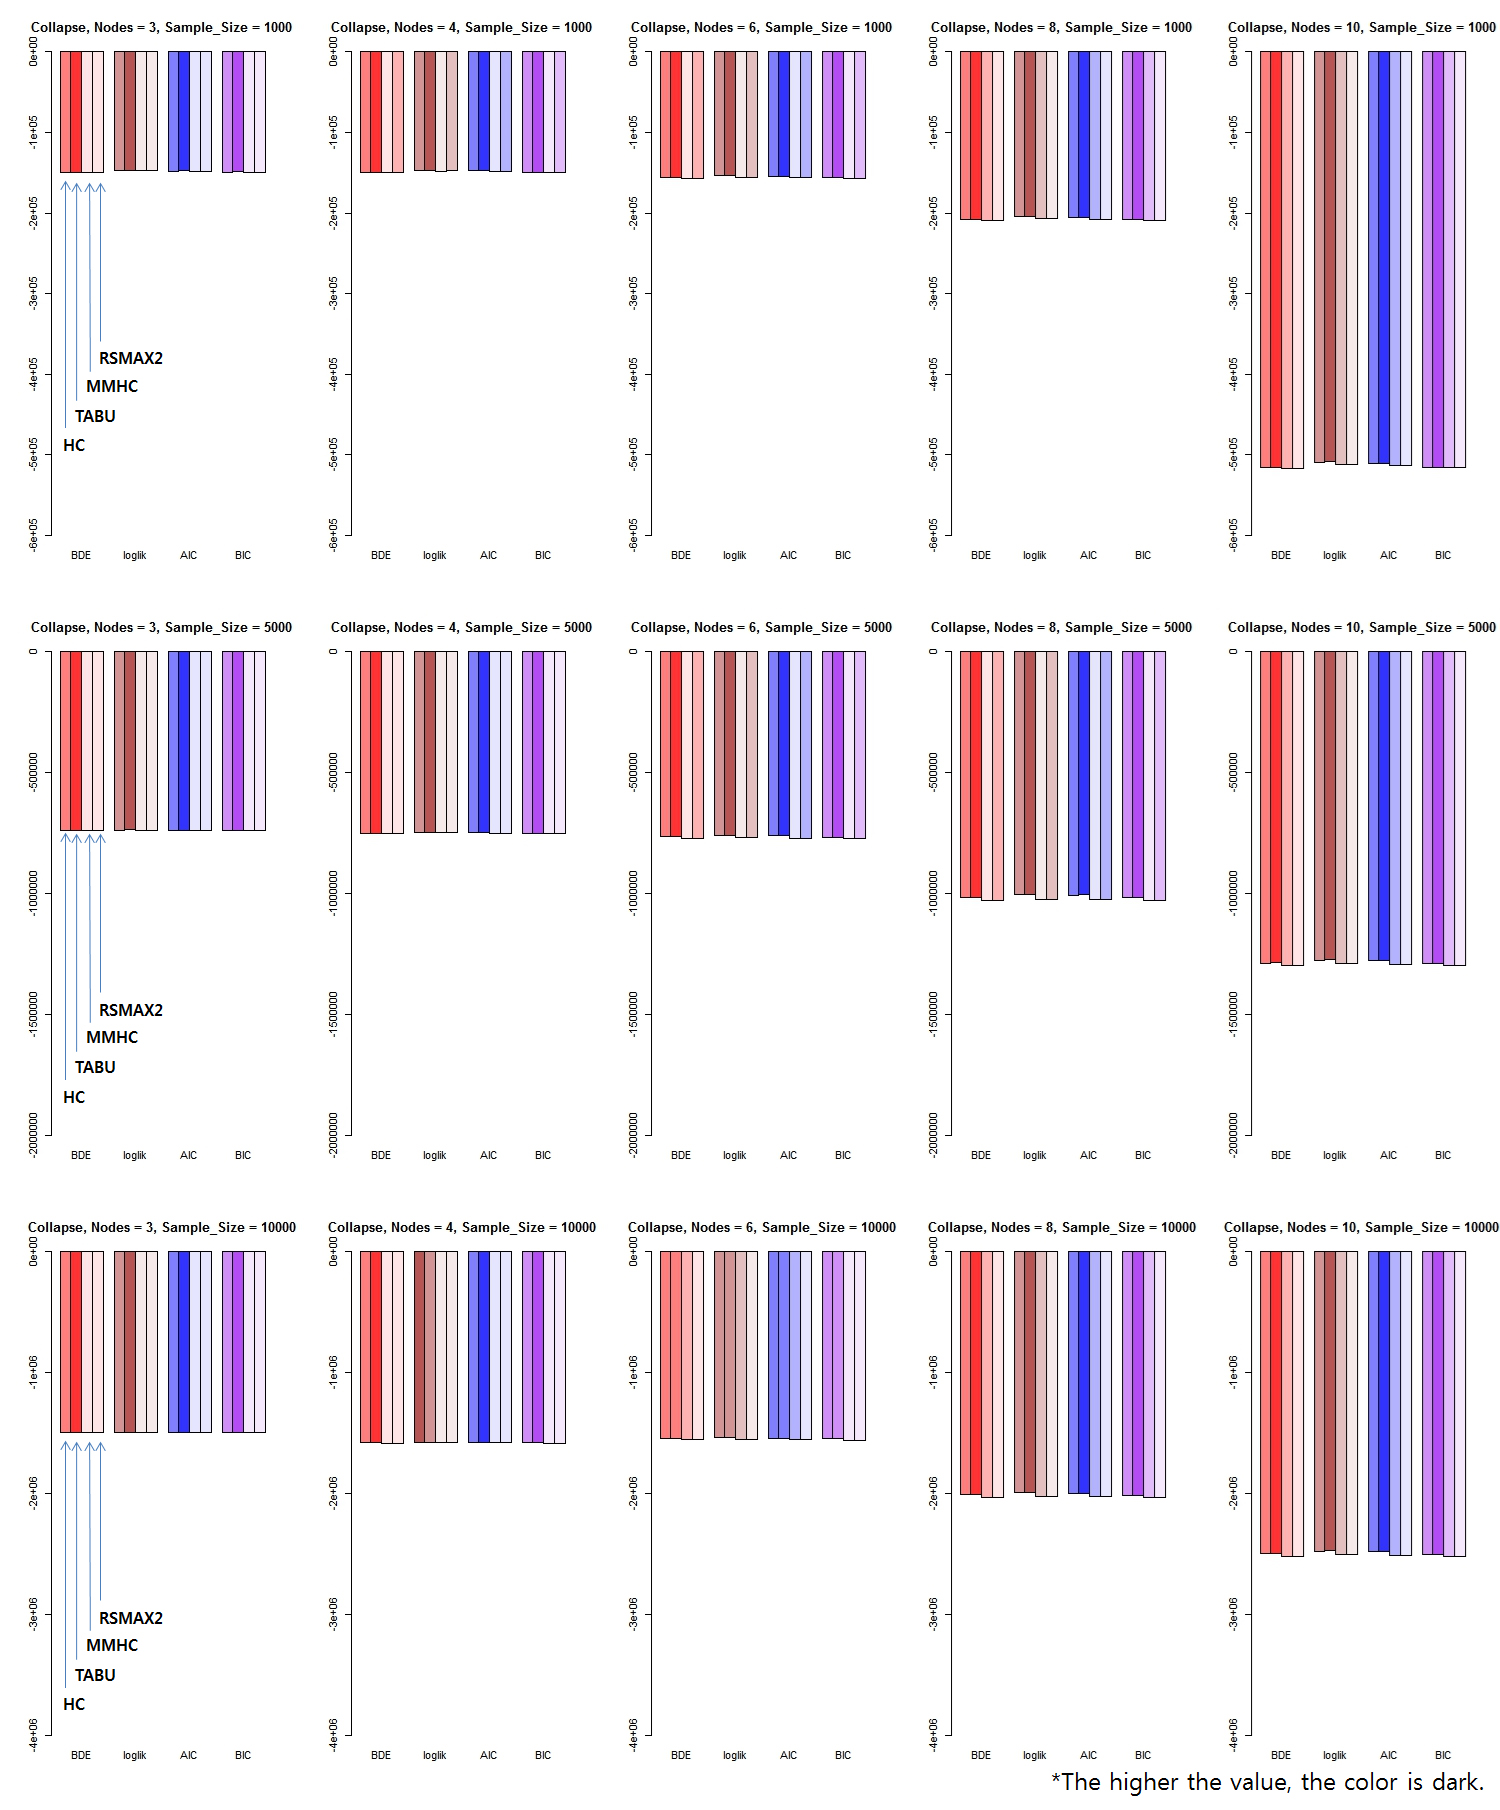
\includegraphics[height=500pt]{01_Collapse_Score}
		\caption{Comparison of scores via Collapse}
	\end{figure}	

	\begin{figure}[p]
	\centering
		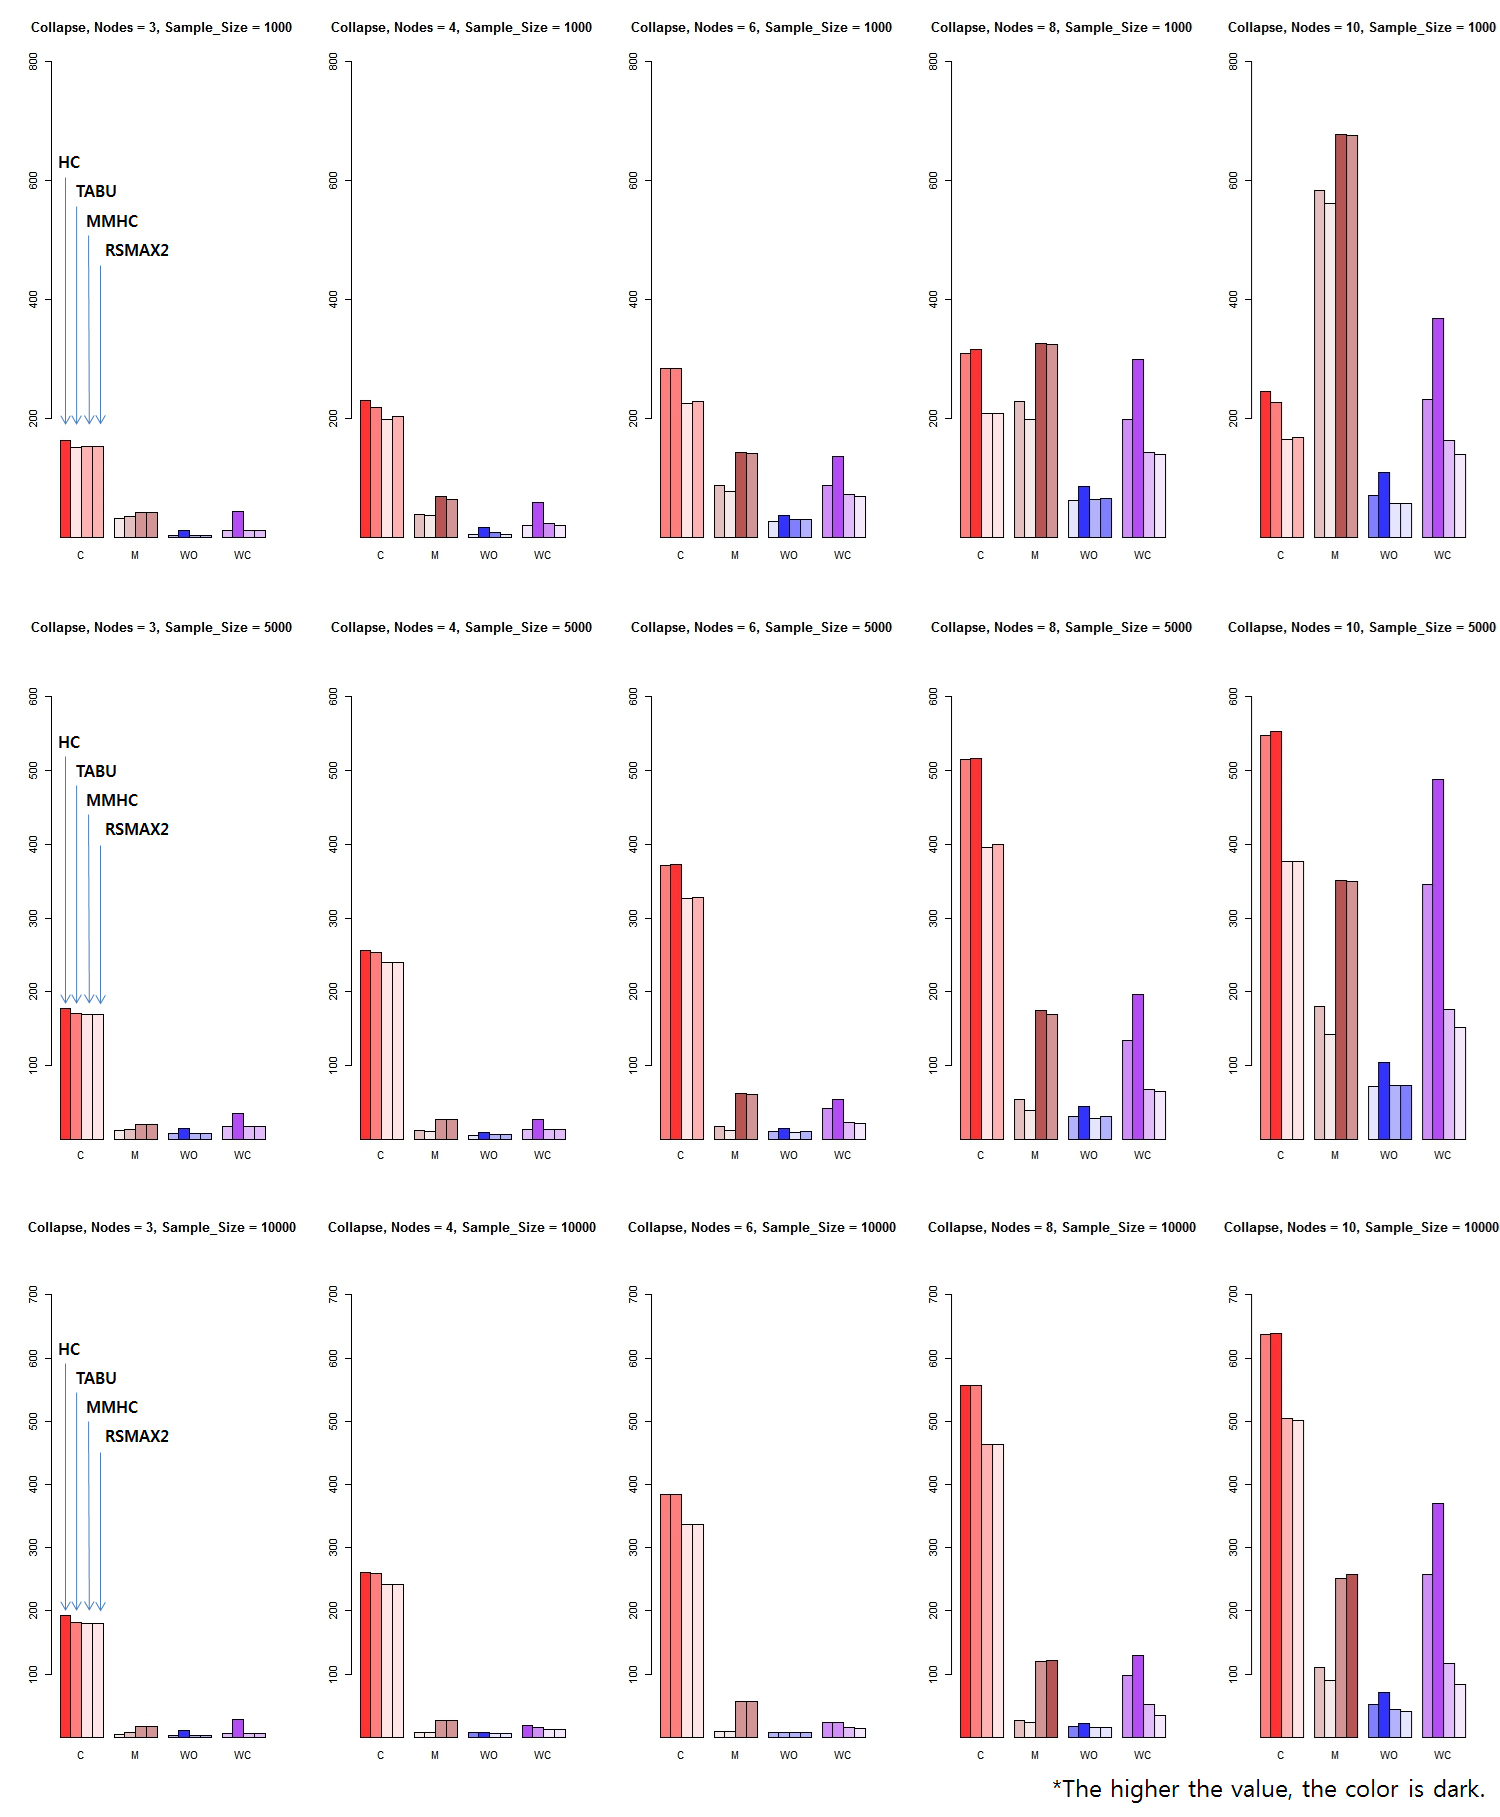
\includegraphics[height=500pt]{01_Collapse_Arcs}
		\caption{Comparison of correct arcs via Collapse}
	\end{figure}	

\newpage{}

